\chapter{Fixed-Length Patterns}
\label{chap:fixpat}


  The set of all permutations, equipped with the pattern ordering, forms an
  infinite graded poset. While much research in this area (and within this
  dissertation) focuses on infinite downsets of this poset, this chapter focuses
  on finite subsets. In particular, we examine the downset induced by a single
  permutation, and investigate the number of distinct patterns. 
  

  In 2003, Herb Wilf raised the question of finding the maximum number of
  distinct patterns which could be contained within a single permutation of
  length $n$, and classifying those permutations which maximize this number. 
  In~\cite{Flynn2007}, the authors showed that the maximum number of patterns
  for a length $n$ pattern is asymptotic to $2^n$, and provided a construction
  which achieves this number. 

  In this chapter we examine the number of distinct patterns of a
  \emph{specified length} which can be contained within a permutation. 
  In the language of posets, Wilf's question asks to find which permutations
  which maximize the size of their downset, while here we seek to maximize the
  \emph{width} of the downset. This chapter can be divided into two parts: in
  the first, we examine the number of $(n-1)$-patterns contained in a random
  permutation of length $n$, and obtain the expectation and variance for this statistic
  by extending a 1945 result of Kaplansky and Wolfowitz~\cite{Kaplansky,
  Wolfowitz}. In the second part, we examine the number of patterns of any
  fixed size within a permutation, and provide a construction which maximizes
  this number. This chapter is based partly on~\cite{me-fixpat}.


% =========================================================================== %
\section{Large Patterns}


  The set of all permutations, equipped with the pattern ordering, forms an
  infinite partially ordered set (see Figure~\ref{prelim:fig:poset}). We focus
  here on the local properties of this poset, namely the number of patterns
  containing and contained in a given pattern. The more general topology of
  this poset was studied by McNamara and
  Steingr\'imsson~\cite{Steingrimsson2013}.

  The set of patterns contained within any fixed permutation forms a partially
  ordered set, in fact a finite downset of the full pattern poset.  To examine
  these downsets, we use a top-down approach: deleting entries one at a time
  from the permutation to obtain the full set of patterns.
  Figure~\ref{fixpat:fig:downsets} shows several examples of these
  downsets\index{downset}. 

  \begin{figure}[t] 
    \centering
    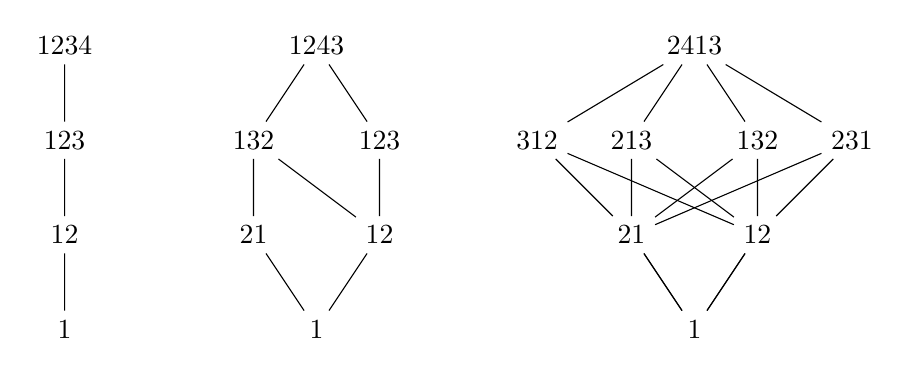
\begin{tikzpicture}
    [scale = .4]
      \node (a1) at (-8,9) {$1234$};
      \node (a2) at (-8,6) {$123$};
      \node (a3) at (-8,3) {$12$};
      \node (a4) at (-8,0) {$1$};
      \draw (a1) -- (a2) -- (a3) -- (a4);

      \node (b1) at (0,9) {$1243$};
      \node (b21) at (-2,6) {$132$};
      \node (b22) at (2,6) {$123$};
      \node (b31) at (-2,3) {$21$};
      \node (b32) at (2,3) {$12$};
      \node (b4) at (0,0) {$1$};
      \draw (b1) -- (b21) -- (b31) -- (b4);
      \draw (b1) -- (b22) -- (b32) -- (b4);
      \draw (b21) -- (b32);

      \node (c1) at (12,9) {$2413$};
      \node (c21) at (7,6) {$312$};
      \node (c22) at (10,6) {$213$};
      \node (c23) at (14,6) {$132$};
      \node (c24) at (17,6) {$231$};
      \node (c31) at (10,3) {$21$};
      \node (c32) at (14,3) {$12$};
      \node (c4) at (12,0) {$1$};
      \draw (c1) -- (c21) -- (c31) -- (c4);
      \draw (c1) -- (c22) -- (c31) -- (c4);
      \draw (c1) -- (c23) -- (c32) -- (c4);
      \draw (c1) -- (c24) -- (c32) -- (c4);
      \draw (c21) -- (c32) --(c22);
      \draw (c23) -- (c31) --(c24);
    \end{tikzpicture}
  \caption{Downsets of 1234, 1243, and 2413} \label{fixpat:fig:downsets}
  \end{figure}

\subsection{Definitions and Notation}

  It will be convenient to establish some machinery for dealing with large
  patterns. Fix $n \geq 2$, let $\pi$ be a permutation of length $n$, and let $\sg$ be an
  $(n-1)$-permutation. If $\sg$ is contained as a pattern within $\pi$, then it
  follows that $1$ can be obtained by deleting one entry from $\pi$, and
  relabelling with respect to order. Similarly, it follows that $\pi$ can be
  obtained by inserting an appropriate entry into $\sg$. We formalize these ideas
  with the following pair of definitions. 


  \begin{definition} \label{fixpat:def:del}
    For any permutation $\pi \in \S_n$, define the function 
    $\del_\pi: [n] \ra \S_{n-1}$, where $\del_\pi(i)$ is the permutation
    obtained by deleting the $i$th entry of $\pi$, and standardizing the
    remaining entries. Let $\del_\pi = \{ \del_\pi(i) : i \in [n]\}$ denote the
    image of $\del_\pi$. 
  \end{definition}

  \begin{definition} \label{fixpat:def:ins}
    For any permutation $\sg \in \S_{n-1}$, define the function
    $\ins_\sg: [n] \times [n] \ra \S_n$, where $\ins_\sg(i,j)$ is the permutation
    obtained by inserting the entry $j - 1/2$ immediately to the left of the
    $i$th entry of $\sg$, and then standardizing the entries. 
    Let $\ins_\sg = \{\ins_\sg(i,j) : i, j \in [n]\}$ denote the image of
    $\ins_\sg$. 
  \end{definition}

  Letting $\pi$ and $\sg$ be an $n$- and $(n-1)$-permutation, respectively, 
  it follows from their definitions that these functions that $\del_\pi$ is the
  set of all $n-1$-patterns contained in $\pi$, and $\ins_\sg$ is the set of
  permutations of length $n$ which contain $\sg$. In addition, these functions satisfy the
  following inverse relationship:
  $$ \del_{\ins_\sg(i,j)}(i) = \sg \text{ and } \ins_{\del_{\pi}(i)}(i, \pi_i).$$


% =========================================================================== %
\section{Plentiful Permutations}
  
    Fix $n \in \Zp$, and let $\pi$ be a permutation of length $n$. Since every pattern
    within $\pi$ can be obtained by deleting elements of $\pi$ one by one,
    the relationship between $\del_\pi$ and $\pi$ can be applied iteratively to
    understand the full downset of $\pi$. It follows directly from the definition
    that $|\del_\pi| \leq n$, and that $|\del_\pi| = n$ if and only if
    $\del_\pi$ is a one-to-one function, i.e., $\del_\pi(i) = \del_\pi(j)$ if
    and only if $i=j$. Before investigating further, we introduce another pair
    of definitions. 

    \begin{definition} \index{permutation!plentiful}
    \label{fixpat:def:plentiful}
      Let $\pi$ be a permutation of length $n$. Say that $\pi$ is \emph{plentiful} if it
      contains $n$ distinct $(n-1)$-patterns. Equivalently, $\pi$ is plentiful
      if and only if $\delpi$ is a one-to-one function. 
    \end{definition}
    
    \begin{definition} \index{bond}
      Let $\pi = \pi_1p_2 \dots \pi_n$ be a permutation, and let $i \in [n-1]$. Say
      that the pair $(\pi_i, \pi_{i+1})$ is a \emph{bond}, of entries of $\pi$ if
      $\pi_i - \pi_{i+1} = \pm 1$. We say that the sequence $(\pi_i, \pi_{i+1}, \dots
      \pi_{i+k-1})$ is a \emph{run} of length $k$ if, for $1 \leq j \leq k-2$,
      the pair $(\pi_{i+j},\pi_{i+j+1})$ is a bond. Denote by $\beta(\pi)$ the
      number of bonds in $\pi$. 
    \end{definition}
  
    Note that runs are necessarily either increasing or decreasing, and that a run
    of length $k$ contains $k-1$ bonds. We can now establish a fundamental
    relationship between bonds and $(n-1)$-patterns. 

    \begin{lemma} \label{fixpat:lem:bonds}
      Let $\pi = \pi_1 \pi_2 \dots \pi_n$. For any $j,k \in [n]$ with $j \neq
      k$, $\del_\pi(i) = \del_\pi(j)$ if and only if $\pi_j$ and $\pi_k$ are
      part of the same run. 
    \end{lemma}
    \begin{proof}
      The forward direction is clear, since removing any element of a run
      simply results in a shorter run. 

      The reverse implication takes a bit more work. Suppose that there exist
      $j,k$ with $1 \leq j < k \leq n$ and $\del_\pi(j) = \del_\pi(k)$. We
      proceed by induction on $k-j$. 

      For the base case, suppose that $k =j+ 1$. Assume first that $\pi_j <
      \pi_{j+1}$, and consider the $j$th entry of $\delpi(j)=\delpi(j+1)$. By
      the definition of $\del$, the $j$th entry of $\delpi(j)$ is
      $\pi_{j+1}-1$, and the same entry in $\delpi(j+1)$ is $\pi_j$. Therefore,
      we see that $\pi_{j+1}-1=\pi_j$, which means that $(\pi_j,\pi_{j+1})$ is
      a bond. Again, the case where $\pi_{j+1}<\pi_j$ follows similarly. 

      Now assume by way of induction that the statement holds when $k=j+m-1$,
      and suppose there exists $1\leq j < k \leq n$ such that $k-j = m$ and
      $\delpi(j)=\delpi(k)$. Assume first that $\pi_j < \pi_{k}$.
      $\delpi(j)=\delpi(k)$ implies, in particular, that the $(k-1)$st entries
      on both sides of the equality are equal.  By definition, the $k-1$ entry
      of $\delpi(j)$ is $\pi_k-1$, while the $k-1$ entry of $\delpi(k)$ is
      either $\pi_{k-1}$ or $\pi_{k-1}-1$. The latter case would imply that
      $\pi_{k-1} = \pi_k$, a contradiction, and so it follows that $\pi_{k-1} =
      \pi_k$. 

      By what has already been proved, $\delpi(k-1) = \delpi(k)$ since these
      entries form a bond. But then $\delpi(j) = \delpi(k) = \delpi(k-1)$, and
      so by the induction hypothesis the entries $(\pi_j \pi_{j+1} \dots
      \pi_{k-1})$ form a run. Finally, $\pi_k - 1 = \pi_{k-1}$ implies that
      $(\pi_j \pi_{j+1} \dots \pi_{k-1} \pi_k)$ is a length $m$ run.  Once
      more, the case where $\pi_j > \pi_k$ follows similarly, and the lemma is
      proved.
    \end{proof}

    The size of the set $\delpi$ then depends entirely on $\beta(\pi)$, since
    each bond decreases by one the number of distinct $(n-1)$-patterns
    contained in $\pi$. This leads to the following theorem, and its immediate
    corollary. 

    \begin{theorem} \label{fixpat:thm:bonds}
      Let $\pi \in \S_n$. Then $|\delpi| = n - \beta(\pi)$. 
    \end{theorem}

    \begin{corollary} \label{fixpat:cor:alldistinct}
      A permutation is plentiful if and only if it contains no bonds. 
    \end{corollary}

    Theorem~\ref{fixpat:thm:bonds} also provides a simple proof of the
    following local property of the permutation pattern poset \index{pattern
    poset}. 

    \begin{corollary} \label{fixpat:cor:n2+1} 
      If $\sg \in \S_{n-1}$, then $|\ins_\sg| = n^2 - 2n + 2 = (n-1)^2 + 1$. In
      other words, every permutation of length $n$ is contained in exactly $n^2 +1$
      $(n+1)$-permutations. 
    \end{corollary}
    \begin{proof}

      By definition, the set $\ins_\sg = \{ins_\sg(j,k) : 1 \leq j , k \leq
      n\}$, so we see that $|\ins_\sg| \leq n^2$.

      Now, a permutation $\pi \in \S_n$ is contained in $\ins_\sg$ more than once
      exactly when $\sg$ can be obtained in more than one way by deleting a entry
      of $\pi$. It follows that $\sg$ is contained in a permutation $\pi \in \S_n$
      more than once exactly when $\ins_\sg(j,k) = \ins_\sg(j\p,k\p)$ where
      $(j,k) \neq (j\p,k\p)$. By the lemma, this happens exactly when the $j$th
      entry of
      $\ins_\sg(j,k)$ is a part of the same run as the $j\p$ entry of
      $\ins_\sg(j\p,k\p)$. We can prevent this from occurring by never inserting
      an element just to the right and directly above or below an existing
      element of $\sg$, as this ensures that any new bonds can be created in
      exactly one way. 

      This eliminates exactly $2(n-1)$ choices for inserting an entry into $\sg$,
      and so therefore $|\ins_\sg| = n^2 - 2(n-1) = (n-1)^2 +1$, and the proof
      is complete.  
    \end{proof}

    
  
% =========================================================================== %
\section{Distribution of the Number of Patterns}
  \label{fixpat:sec:delpi}

  We now consider let $\pi$ be a (uniformly) randomly \index{random} chosen
  permutation of length $n$, and examine the distribution of the statistic
  $|\delpi|$. The correlation presented in Theorem~\ref{fixpat:thm:bonds}
  allows us to investigate this distribution by analyzing the distribution of
  bonds. This distribution has been examined previously in other contexts, most
  notably by Kaplansky and Wolfowitz~\cite{Kaplansky, Wolfowitz}. In this
  section we extend their asymptotic results by finding \emph{exact} values for
  the expectation and variance of $\beta(\pi)$, and therefore of $|\delpi|$. 

  Throughout this section, fix $n$ and let $\dtan$ and $\btan$ be random
  variables denoting the number of distinct $(n-1)$-patterns and the number of
  bonds in a random permutation of length $n$, respectively.  Our primary tool
  in this investigation will be multivariate generating functions, but first we
  note that $\Ex{\dta}$ can be obtained directly using results from the
  previous section. \index{generating function!multivariate}

  \begin{proposition} \label{fixpat:prop:easyexpectation}
    The expectation of $\dta$ is equal to $n - \frac{2(n-1)}{n}$, which
    approaches $n-2$ as $n$ increases. 
  \end{proposition}
  \begin{proof}
    By the definition of expectation, we have 
    $$ \Ex{\dta} = \frac{\sum_{\pi \in \S_n} |\delpi| }{n!}. $$
    The proposition then follows immediately from
    Corollary~\ref{fixpat:cor:n2+1} and the identity
    $$ (n^2 - 2n + 2) (n-1)! = \left(n - \frac{2(n-1)}{n}\right) n!.$$
  \end{proof}


\subsection{Generating Functions}

  Generating functions allow us to go several steps further, and obtain
  higher moments for the distributions of these variables. It follows from
  Theorem~\ref{fixpat:thm:bonds} and the linearity of expectation
  \index{expectation!linearity} that 
  $$ \Ex{\dta} = n - \Ex{\bta}.$$
  Therefore we can translate the distribution of $\bta$ to that of $\dta$. 
  We start by building a multivariate generating function which keeps track
  of the distribution of bonds throughout all permutations. We use a method
  similar to the cluster method of Goulden and Jackson~\cite{gouldenjackson1,
  gouldenjackson2}, described by Noonan and Zeilberger~\cite{Noonan1999}. Note
  that this generating function converges nowhere, but still yields useful
  algebraic information. 

  \begin{theorem} \label{fixpat:thm:genfcn}
    Let $a_{n,k}$ be the number of permutations of length $n$ which contain
    exactly $k$ bonds, and let $a_{0,0} = 1$. Then the numbers $a_{n,k}$ have
    the following generating function
    $$ \sum_{n \geq 0} \sum_{k \geq 0} a_{n,k} z^n u^k = 
      \sum_{m \geq 0} m! \left(z + \frac{2z^2(u - 1)}{1 - z(u-1)}\right)^m.$$
    Denote this function by $f(z,u)$. 
  \end{theorem}
  \begin{proof}
    First we construct a related generating function, then translate it into
    ours using the technique of inclusion-exclusion. 
    Say that a bond in a permutation can be arbitrarily \emph{marked}, and then a  
    \emph{marked permutation} is one in which each bond is either marked or
    unmarked.  Let $b_{n,k}$ be the number of permutations of length $n$ which contain
    exactly $k$ marked bonds. For example, $b_{n,0} = n!$, since every
    permutation can be written with no bonds marked, and no permutation is
    counted more than once. Similarly, $b_{n,n-1} = 1$, since the only
    marked permutation with $n-1$ marked bonds is the decreasing permutation
    with all of its bonds marked. 

    Let 
    $$ g(z,u) := \sum_{n \geq 0}\sum_{k \geq 0} b_{n,k}z^n u^k. $$ 
    This generating
    function is easier to construct, as we can build a permutation of length $n$ with
    $k$ marked bonds by first specifying our marked runs, then permuting
    these runs with the remaining entries. The benefit to this method is that
    we don't have to worry about bonds forms between these runs, as we have
    already specified which ones are marked. A marked run of length $j$
    can be either ascending or descending, and contains $j-1$ bonds. 
    It follows that 

    $$ g(z,v) = \sum_{m \geq 0}
        m! \left(z + \frac{2z^2v}{1 - zv} \right)^m.$$

    Now, we can use this generating function to obtain $f(z,u)$. The variable
    $v$ keeps track of marked bonds, while $u$ keeps track of all bonds.
    Since every bond can either be marked or unmarked, it follows that by
    substituting $u$ for $v + 1$ we can translate $f(z,u)$ to $g(z,v)$.
    Therefore, we have the relation $f(z,v+1) = g(z,v)$, from which we see
    that 
    $$ f(z,u) = g(z,u-1) = 
      \sum_{m \geq 0} m! \left(z + \frac{2z^2(u-1)}{1 - z(u-1)} \right)^m.$$
  \end{proof}

  The following corollary is immediate, and follows from the relationship
  between $\dta$ and $\bta$. 
    
  \begin{corollary} \label{fixpat:cor:gfn2}
    Let $d_{n,k}$ denote the number of permutations of length $n$ containing
    exactly $k$ distinct $(n-1)$ patterns, and let $d_{0,0} = 1$. Then 
    $$ h(z,u) :=  \sum_{n \geq 0}\sum_{ k \geq 0} h_{n,k} z^n u^k = 
      \sum_{m \geq 0}  m! \left( zu + 
      \frac{2zu^2 (1/u - 1)}{1 - zu(1/u - 1)}\right)^m.$$
  \end{corollary}
  \begin{proof}
    Since $\dta = n - \bta$, it follows that $h(z,u) = f(zu, 1/u)$. 
  \end{proof}

  The remainder of this section will consist of the analysis of the function
  $F(z,u)$, and the translation of this analysis into facts about
  permutations. 
  First, we compute the number of permutations which have no bonds (and
  are therefore plentiful). 

  \begin{proposition} \label{fixpat:cor:chessboard}
    Let $b_n$ be the number of permutations of length $n$ with no bonds. Then 
    $$ \begin{aligned} 
     \sum_{n \geq 0} b_n z^n 
       &= \sum_{m \geq 0} m! z^m \frac{(1 - z)^m}{(1 + z)^m} \\
       &= 1 + z + 2z^4 + 14z^5 + 90z^6 + 646z^7 + 5242z^8 + \dots 
    \end{aligned} $$
  \end{proposition}
  \begin{proof}
    This follows immediately by setting $u = 0$ in $f(z,u)$. 
  \end{proof}

  The numbers $b_n$ in Corollary~\ref{fixpat:cor:chessboard} are 
  \OEIS{A002464}. These numbers are also equal to the number of ways of
  placing $n$ non-attacking kings on an $n \times n$ chessboard with one king
  per each row and column, as can be seen by plotting the permutations. It
  was shown in~\cite{Tauraso2006} that this sequence is asymptotic to
  $n!/e^2$, and so Corollary~\ref{fixpat:cor:alldistinct} implies the
  following corollary. 

  \begin{corollary}
    The probability that a randomly selected $n$ permutation is plentiful tends
    to $1/e^2$ as $n$ tends to infinity. 
  \end{corollary}

  In addition to exact results, we can use the function $f(z,u)$ to determine
  the \emph{expected} \index{expectation} number of bonds within a randomly
  selected permutation of length $n$, Using techniques described in
  Chapter~\ref{chap:prelim} and in \cite{flajolet}. 
  
  
  \begin{theorem} \label{fixpat:thm:exvar}
    The expectation and variance of the random variable $\btan$ are as
    follows:
    $$ \begin{aligned}
        \Ex{\btan} &= 2\frac{(n-1)}{n} \\
        \Var{\btan} &= 4\frac{(n-2)^2}{n(n-1)} + 2\frac{n-1}{n} -
        4\frac{(n-1)^2}{n^2} . 
        \end{aligned} $$
  \end{theorem}
  \begin{proof}
    The expectation is obtained by taking the partial derivative with respect
    to $u$, then plugging in $u = 0$ as shown below. 

    $$ \begin{aligned}
      \sum_{n\geq 0}\Ex{\btan}z^n 
        &= \frac{\partial_u f(z,u) \big|_{u=0}}{n!} \\
        &= \sum_{n \geq 0} 2 (n-1)! \cdot (n-1) z^n. 
      \end{aligned}$$
    
    The second factorial moment $\Ex{\btan(\btan - 1)}$ can be computed from
    the generating function as follows:
    
    $$ \sum_{n \geq 0} \Ex{\btan(\btan - 1)}z^n 
      = \frac{\partial_u^2 f(z,u) \uisone}{n!}.$$
    
    The variance can then be computed using linearity of expectation:
    \index{expectation!linearity}
    $$ \Var{\btan^2} = \Ex{\btan^2} - \Ex{\btan}^2 
      = \Ex{\btan(\btan - 1)} + \Ex{\btan} - \Ex{\btan}^2.$$
    
    From here, a tedious and technical computation finishes the proof. 
  \end{proof}

  Higher moments can be computed iteratively. 
  The relationship between the variables $\btan$ and $\dtan$ immediately
  provides the corresponding expectation and variance for $\dtan$. Taking the
  limit as $n \ra \infty$ gives asymptotic values for this distribution,
  which leads to the results found in~\cite{Kaplansky, Wolfowitz}. We
  summarize these ideas in the following corollaries. 

  \begin{corollary}\label{fixpat:cor:exvar}
    The expectation and variance for the variable $\dtan$ are as follows:
    $$ \begin{aligned} 
       \Ex{\btan} &= n - \frac{2(n-1)}{n} \\
        \Var{\btan} &= 4\frac{(n-2)^2}{n(n-1)} + 2\frac{n-1}{n} -
        4\frac{(n-1)^2}{n^2}. 
        \end{aligned} $$
  \end{corollary}

  \begin{corollary}
    For large $n$, we have that 
    $$ \Ex{\btan} \sim n - 2 \text{ \quad and \quad }
      \Var{\btan} \sim 2.$$
  \end{corollary}


\section{Patterns of Other Sizes}
  \label{fixpat:sec:othersizes}
  
  In this section, we examine the number of distinct $(n-k)$-patterns contained
  in a permutation of length $n$. For a given permutation of length $n$ $\pi$, $\delpi$ denotes
  the image of the function $\delpi$, which is exactly the set of
  $(n-1)$-patterns contained in $\pi$. The following definitions generalize
  the Definitions~\ref{fixpat:def:del} and~\ref{fixpat:def:plentiful}. 

  \begin{definition} \label{fixpat:def:delpik}
    Let $S = \{i_1, i_2, \dots i_k\} \subseteq [n]$, with $i_1 < i_2 < \dots
    < i_k$. We denote by $\delpi(S)$ the permutation obtained by deleting the
    entries in positions $i_1, \dots i_k$, and standardizing the remaining
    entries. Denote by $\delpik$ the set of all permutations which can be
    obtained by deleting $k$ entries from $\pi$ and standardizing. 
  \end{definition}

  \begin{definition} \label{fixpat:def:kplentiful}
    Say that a permutation of length $n$ $\pi$ is \emph{$k$-plentiful} if it has the maximal
    number of distinct $(n-k)$-patterns, i.e., if 
    $$|\delpik| = \binom{n}{k}.$$
  \end{definition}

\subsection{Characterizing k-plentiful Permutations}

  We seek to characterize those permutations which are $k$-plentiful, for an
  arbitrary $k \in [n]$. In Section~\ref{fixpat:sec:delpi} we found that a
  permutation is plentiful if and only if it contains no bonds. By generalizing
  our notion of bonds, we obtain an analogous result here. 

  \begin{definition} \label{fixpat:def:gap}
    Let $\pi = \pi_1 \pi_2 \dots \pi_n \in \S_n$. For any two integers $i,j
    \in [n]$, define the \emph{distance} $d_\pi(i,j)$ between $i$ and $j$ to be 
    $$ d_\pi(i,j) = |i - j| + |\pi_i - \pi_j|.$$
    The \emph{minimum gap} of $\pi$, denoted by $\Gam(\pi)$, is defined to be
    the minimum distance between any two entries. Formally:
    $$ \Gam(\pi) = \min\{ d_\pi(i,j) : 1 \leq i, j \leq n \}.$$
  \end{definition}

  If we plot a permutation $\pi$, then the function $d_\pi$ is just the usual
  taxicab metric on $\{(i, \pi_i) : 1 \leq i \leq n\} \subset \mathbb{R}^2$. 
  It is easy to see that $(\pi_i, \pi_j)$ is a bond if and only if $d_\pi(i,j)
  = 2$. It follows then that $\pi$ is plentiful if and only if $\Gam(\pi) \geq 3$.
  This idea allows us to generalize Corollary~\ref{fixpat:cor:alldistinct}.  We
  start with one more definition, and a simple lemma which will prove useful. 

  \begin{definition} \label{fixpat:def:span}
    Let $\pi = \pi_1 \pi_2 \dots \pi_n \in \S_n$ and let $i,j \in [n]$ with $i
    < j$. The \emph{span} of the indices $i$ and $j$, denoted
    $\pspan_\pi(i,j)$, is defined as the set of indices corresponding to
    entries which are between $(i,\pi_i)$ and $(j,\pi_j)$ either horizontally
    and vertically. Formally, when $\pi_i < \pi_j$ we have
    $$ 
    \pspan_\pi(i,j) = \{k : i < k < j\} \cup \{k : \pi_i < \pi_k < \pi_j \}.
    $$
    The case when $\pi_i > \pi_j$ is defined analogously. 
  \end{definition}
  

  \begin{lemma} \label{fixpat:lem:span}
    Let $\pi \in \S_n$ be such that $\Gam(\pi) = m$, and let $i,j$ be such that
    $d_\pi(i,j) = m$. Then $|\pspan_\pi(i,j)| = m-2$. Further, deleting one
    entry can reduce the minimum gap by at most one, i.e., $\Gam(\delpi(k))
    \geq k-1$ for all $k \in [n]$. 
  \end{lemma}
  \begin{proof}
    Clearly $|\pspan_\pi(i,j)| \leq m-2$, since otherwise this would contradict
    $\Gam(\pi) = m$. The only way in which $|\pspan_\pi(i,j)|$ could be less
    than $k-2$ is if there exists an entry $\pi_k$ which lies between
    $(i,\pi_i)$ and $(j,\pi_j)$ both vertically and horizontally. However, this
    would imply that $d_\pi(i,m) < d_\pi(i,j) = m-2$, which contradicts the
    minimality of $d_\pi(i,j)$. Therefore, $|\pspan_\pi(i,j)| = m-2$. 

    For the second part, note that the only way that deleting a single entry
    could reduce the minimum gap by more than one is if that entry lies between
    two minimally separated entries. However, we have just seen that no such
    entry exists. 
  \end{proof}

  We are now able to give a partial characterization of the $k$-plentiful
  permutations in the following generalization of
  Corollary~\ref{fixpat:cor:alldistinct}. 

  \begin{theorem} \label{fixpat:thm:kplentiful}
    A permutation $\pi$ is $k$-plentiful if and only if $\Gam(\pi) \geq k+2$. 
  \end{theorem}
  \begin{proof}
    First let $\pi = \pi_1 \pi_2 \dots \pi_n$ be a $k$-plentiful permutation, and
    assume by way of contradiction that $\Gam(\pi) = m < k+2$. Let $i<j$ be
    such that $d_\pi(i,j) = m$. By Lemma~\ref{fixpat:lem:span}, we have that
    $\pspan_\pi(i,j) = \{s_1, s_2, \dots s_{m-2}\}$. Let $\sg =
    \delpi(\pspan_\pi(i,j) \in \S_{n-m+2}$, the permutation obtained by
    removing the entries with indices $s_i$ and standardizing the remaining
    entries. If follows then that $\Gam(\sg) = 2$ and so $\sg$ has a bond
    $(\sg_i, \sg_j)$ and is therefore not plentiful. It follows then that
    $\del_\sg(i) = \del_\sg(j)$, and so there are two sets of indices $S$ and
    $S\p$ for which $\del_\pi(S) = \del_\pi(S\p)$. Therefore $|\delpik| <
    \binom{n}{k}$, contradicting the plentifulness of $\pi$. 

    For the other direction, we proceed using induction.
    We have already shown that the theorem holds when $k=1$
    (Corollary~\ref{fixpat:cor:alldistinct}), so let $k>1$ and assume that the
    statement holds for all positive integers less than $k$.
    Let $\pi \in \S_n$ be such that $\Gam(\pi) \geq k+2$. We know by induction
    that this permutation is $m$-plentiful for all $1 \leq m < k$. 

    Suppose by way of contradiction that $\sg \in \S_{n - k}$ can be obtained
    by deleting two different sets of entries from $\pi$. That is, suppose that
    there exist $A = \{a_1, a_2, \dots a_k\} \neq B = \{b_1, b_2, \dots
    b_k\}$, with $a_i < a_j$ and $b_i < b_j$ for $i < j$, such that $\delpi(A)
    = \delpi(B) = \sg$. Claim that $A \cap B = \emptyset$. To see this, suppose
    that $a_i = b_j$, and note that since $A - \{a_i\} \neq B - \{b_j\}$, 
    $\sg$ is contained in $\delpi(a_i)$ in two different ways. However, by
    Lemma~\ref{fixpat:lem:span}, $\Gam(\delpi(a_i)) \geq k + 1$, and so by
    induction $\delpi(a_i)$ is $(k-1)$-plentiful, a contradiction. Therefore $A$ and
    $B$ must be disjoint. 

    Assume without loss of generality that $a_1 < b_1$. Let $j \in [n]$ be the
    smallest integer such that $j > a_1$ but $j \notin A$. Since $\delpi(A) =
    \delpi(B) = \sg = \sg_1 \sg_2 \dots \sg_{n-k}$, it follows that the
    entries $p_{a_1}$ will move to fulfill the role of $\sg_{a_1}$ once the $B$
    entries are deleted. However, the entry $a_j$ will also move to fulfill
    this role once the $A$ entries are deleted. However, this implies that
    every entry in the span of $\pi_{a_1}$ and $\pi_{j}$ must be deleted, but
    there must be at least $k$ such entries by Lemma~\ref{fixpat:lem:span}.
    Therefore, $A$ must contain $a_1$ and $k$ additional entries, contradicting
    $|A| = k$ and proving the theorem. 
  \end{proof}



\subsection{Constructing k-plentiful Permutations}

  It is not immediately obvious that there exist permutations with arbitrarily
  large minimum gaps. In~\cite{Flynn2007}, the authors constructed a
  permutation of length $(k-1)^2$ which has a minimum gap equal to $k$. 
  We conclude this section with a construction that gives a slightly smaller
  permutation which achieves the same gap size, and prove that this
  construction is the best possible. 

  \begin{figure}[t]
    \centering
    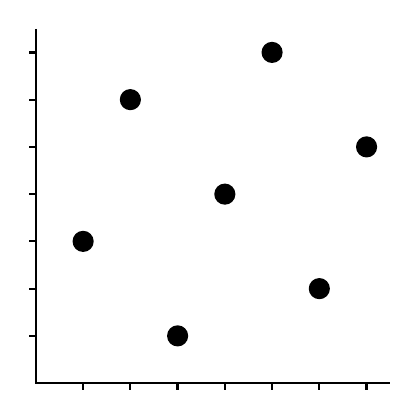
\begin{tikzpicture}
      [scale = .3, line width = .8pt]
      \draw (0,15) -- (0,0) -- (15,0);
      \foreach \num in {2, 4,..., 14}
      {
        \draw (\num, 0) -- (\num, -.3);
        \draw (0, \num) -- (-.3, \num);
      }
      \foreach \y [count = \x] in {3,6,1,4,7,2,5}
        \draw[fill = black] (2*\x,2*\y) circle (4mm);
    \end{tikzpicture} \hspace{4pc}
    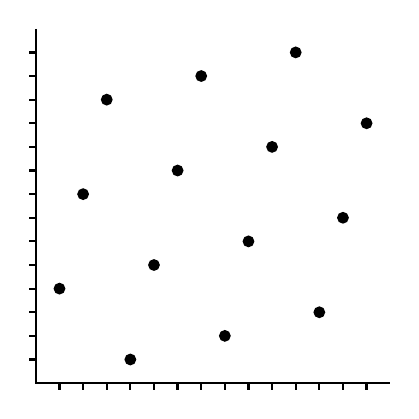
\begin{tikzpicture}
      [scale = .3, line width = .8pt]
      \draw (0,15) -- (0,0) -- (15,0);
      \foreach \num in {1,..., 14}
      {
        \draw (\num, 0) -- (\num, -.3);
        \draw (0, \num) -- (-.3, \num);
      }
      \foreach \y [count = \x] in {4,8,12,1,5,9,13,2,6,10,14,3,7,11}
        \draw[fill = black] (\x,\y) circle (2mm);
    \end{tikzpicture}
    \caption{The plots of the permutations $\Theta^{(4)}$ and $\Theta^{(5)}$.}
    \label{fixpat:fig:thetan}
  \end{figure}

  \begin{definition}
    Let $\pi \in \S_{(k-1)^2}$ be defined by 
    $$\pi_{i(k-1) + j + 1} = i + j(k-1) + 1, \quad 0 \leq i,j \leq k-2.$$
    Then let $\Theta^{(k)} \in \S_{(k-1)^2 - 2}$ be defined by removing the first
    and last entries of $\pi$. 
  \end{definition}



  
  The permutations $\Theta^{(4)}$ and $\Theta^{(5)}$ are shown in
  Figure~\ref{fixpat:fig:thetan}. It is clear from the figure, and can be
  shown from the definition (with some tedious but simple calculation) that
  $\Gam(\Theta^{(k)}) = k$. It also follows that $\Theta^{(k)}$ is an
  involution, and its reverse is equal to its complement, so its orbit
  under the automorphism group of the pattern poset consists of only two
  elements. 

  % \begin{figure}[t]
  %   \centering
  %   \begin{tikzpicture}
  %     [scale = .3, line width = .8pt]
  %     \draw (0,15) -- (0,0) -- (15,0);
  %     \foreach \num in {2, 4,..., 14}
  %     {
  %       \draw (\num, 0) -- (\num, -.3);
  %       \draw (0, \num) -- (-.3, \num);
  %     }
  %     \foreach \y [count = \x] in {3,6,1,4,7,2,5}
  %       {\draw[fill = black] (2*\x,2*\y) circle (4mm);
  %       \draw (2*\x + 4, 2*\y - 1.33) -- (2*\x +2, 2*\y +3.33) -- 
  %             (2*\x - 4,  2*\y + 1.33) -- (2*\x - 2 ,2*\y -3.33) -- cycle;}
  %   \end{tikzpicture} \hspace{4pc}
  %   \caption{The tiling associated to $\Theta^{(4)}$.}
  %   \label{fixpat:fig:tiling}
  % \end{figure}


  By embedding a permutation $\pi$ into the plane, the function $d_\pi$ can be
  extended to the usual taxicab metric $d_1$ on $\mathbb{R}^2$. If $\pi$ has a
  minimum gap size of $k$, then $\pi$ defines a tiling of the plane with angled
  bricks of uniform size and centered on the points of $\mathbb{Z}^2$. It
  is clear that a minimal such permutation will correspond to a maximal tiling
  of this form, with the property that no two centers lie on the same
  horizontal or vertical line. There are exactly two such tilings, corresponding to
  the permutation $\Theta^{(k)}$ and its reverse.
  % (see Figure~\ref{fixpat:fig:tiling}). 
  We summarize this in the following theorem. 

  \begin{theorem} \label{fixpat:thm:tiling}
    The permutation $\Theta^{(k)}$ and its reverse are the shortest
    permutations with minimum gap size equal to $k$. 
  \end{theorem}

  We end this chapter with one last theorem, generalizing
  Theorem~\ref{fixpat:thm:bonds}.

  \begin{theorem} \label{fixpat:thm:gappairs}
    Let $\pi \in \S_{n}$ have $\Gam(\pi) = k + 1$, and let $p_k$ be the number
    of pairs $(i,j)$ such that $d_\pi(i,j) = k$. Then 
    $$ | \delpik | = \binom{n}{k} - p_k.$$
  \end{theorem}
  \begin{proof}
    Let $\pi \in \S_n$ be such that $\Gam(\pi) = k+1$, and let $i,j \in [n]$ be
    such that $d_\pi(i,j) = k+1$ (i.e., $|\pspan_\pi(i,j)| = k-1$). If we let
    $S = \pspan_\pi \cup i$ and $S\p = \pspan_\pi \cup j$, we see that
    $\delpi(S) = \delpi(S\p)$, and so 
    $$\delpik \leq \binom{n}{k} - p_k. $$
    To show equality, let $A = \{a_1, a_2, \dots a_k\} \neq B = \{b_1, b_2,
    \dots b_k\}$, with $a_i < a_j$ and $b_i < b_j$ when $i < j$, and suppose
    that $\delpi(A) = \delpi(B)$. 
    
    Claim that $|A \cap B| = k-1$, i.e., that the two sets differ by exactly
    one element. .  Suppose first that $a_1 \neq b_1$, and let $s$ be the
    smallest integer greater than $a_1$ such that $s \notin A$. Then, as in the
    proof of Theorem~\ref{fixpat:thm:kplentiful}, we have $d_\pi(a_1, s) = k+1$, and
    $A - {a_1} = B - {b_1} = \pspan_\pi(a_1, s)$.  In the case where $a_1 =
    b_1$, let $\pi\p = \delpi(a_1)$, $A\p = A - \{a_1\}$, and $B\p = B -
    \{b_1\}$. Since $\del_{\pi\p} (A\p) = \del_{\pi\p}(B\p)$, by
    Lemma~\ref{fixpat:lem:span} and Theorem~\ref{fixpat:thm:kplentiful} imply that that
    $\Gam(\pi\p) = k$. We now find that either $a_2 = b_2$ or $A\p - \{a_2\} =
    B\p - \{b_2\}$. Iterating this argument shows that the two sets differ by
    at most one element. 

    Finally, let $i,j$ be such that $a_i \in A - B$ and $b_j \in B - A$. It
    follows then that $ A-\{a_i\} = B - \{b_j\} - \{\pspan_\pi(i,j) \}$. But
    since their span has size $k-1$, their distance must be equal to $k+1$,
    an element in between them both horizontally and vertically would
    contradict the size of the minimum gap. Thus, each pair $i,j$ for which
    $d_\pi(i,j) = k+1$ reduces the number of $(n-k)$-patterns by exactly one,
    which completes the proof. 
  \end{proof}





    

      

